\section{Alternative Design (to delete?)} 
\label{sec:Design Alternative}
In the first stages of the realization of this work, the CBCE configuration was taken into account as a valid alternative to the differential balun in Section \ref{sec:Schematic_Design} but it was eventually discarded, not due to any shortcomings, but rather because of very low output impedances, for which the reason is believed to be the low number of fingers, that might would have complicated the design matching network.
The proposed schematic is shown in Figure \ref{fig:SchematicCBCE} and its MaxGain in Figure \ref{fig:SchematicCBCE_measureMaxGain}.

\begin{figure}[hbt!]
    \centering
    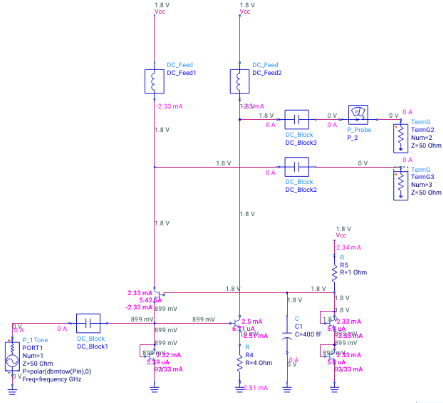
\includegraphics[width=0.75\linewidth]{Design_figures/CBCE/SchematicCBCE.PNG}
    \caption{CBCE active balun configuration}
    \label{fig:SchematicCBCE}
\end{figure}
%%%%%%%%%%%%%%%%%%

\begin{figure}[H]
    \centering
    \begin{subfigure}[b]{0.48\linewidth}
        \centering
        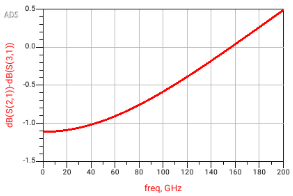
\includegraphics[width=\linewidth]{Design_figures/CBCE/SchematicCBCE_measureAmplitudeImbalance.PNG}
        \caption{}
        \label{fig:SchematicCBCE_measureAmplitudeImbalance}
    \end{subfigure}
    \hfill
    \begin{subfigure}[b]{0.48\linewidth}
        \centering
        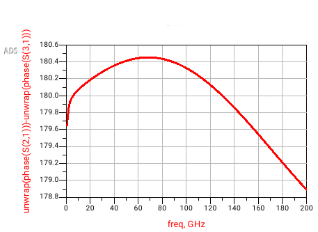
\includegraphics[width=\linewidth]{Design_figures/CBCE/SchematicCBCE_measurePhaseImbalance.PNG}
        \caption{}
        \label{fig:SchematicCBCE_measurePhaseImbalance}
    \end{subfigure}
    \caption{Measure of (a) Ampltude imbalance and (b) Phase imbalance of the schematic CBCE active balun configuration in the D-band.}
    \label{fig:placeholder}
\end{figure}
%%%%%%%%%%%%%%%%%%
The schematic design imbalance performances were tuned out by the degeneration resistor placed at the Common emitter transistor \cite{Transformer_matched_gilbert_mixer} and the results presented are the tradeoff between amplitude and phase imbalance. having said this, the schematic design in Figure \ref{fig:SchematicCBCE}  present and amplitude imbalance, Figure \ref{fig:SchematicCBCE_measureAmplitudeImbalance}),  of $-0.3 \pm 0.8$ with an offset between $S_{21}$ and $S_{31}$ of $-0.3$dB while the phase imbalance, Figure \ref{fig:SchematicCBCE_measurePhaseImbalance}, is within $179.7^{\circ} \pm 0.8 ^{\circ}$.
From this simulation it is possible to foresee the potential of this topology to act as a D band balun \textcolor{red}{but a carefull examination is to be taken on the degeneration resistor as a very low value is most likely to be needed.}
%%%%%%%%%%%%%%%%%%%%%%%%%%%%%
\\
A first layout realization in Figure \ref{fig:LayoutCBCE}, with the respective simulations were also performed.
The single stage CBCE, in terms of amplitude balance, does surpass the two-stage differential balun of this work, as it is shown in figure(\ref{fig:LayoutCBCE_measureAmplitudeImbalance}). The phase imbalance is far worse although, this is partially attributed to the offset created by the different transmission line lengths and hence it can be adjusted
%%%%%%%%%%%%%%%%%%
\begin{figure}[H]
    \centering
    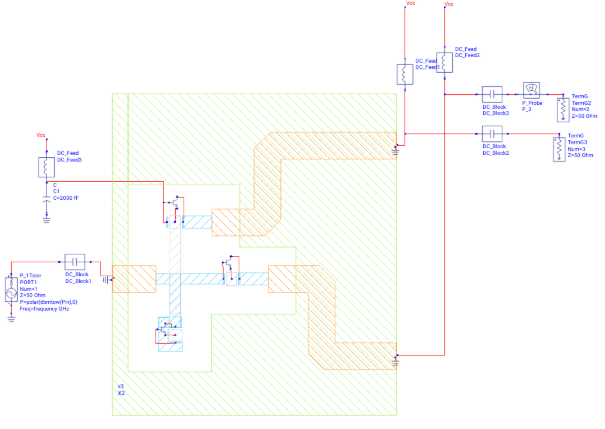
\includegraphics[width=1\linewidth]{Design_figures/CBCE/LayoutCBCE.PNG}
    \caption{Layout of the CBCE active balun configuration}
    \label{fig:LayoutCBCE}
\end{figure}
%%%%%%%%%%%%%%%%%%
%%%%%%%%%%%%%%%%%%
\begin{figure}[H]
    \centering
    \begin{subfigure}[b]{0.48\linewidth}
        \centering
        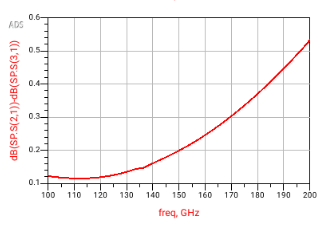
\includegraphics[width=\linewidth]{Design_figures/CBCE/LayoutCBCE_measureAmplitudeImbalance.PNG}
        \caption{}
        \label{fig:LayoutCBCE_measureAmplitudeImbalance}
    \end{subfigure}
    \hfill
    \begin{subfigure}[b]{0.48\linewidth}
        \centering
        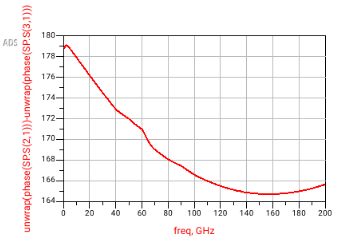
\includegraphics[width=\linewidth]{Design_figures/CBCE/LayoutCBCE_measurePhaseImbalance.PNG}
        \caption{}
        \label{fig:LayoutCBCE_measurePhaseImbalance}
    \end{subfigure}
    \caption{Measure of (a)Amplitude imbalance and (b) Phase imbalance of the layout CBCE active balun configuration simulated in the D-band.}
    \label{fig:placeholder}
\end{figure}

%%%%%%%%%%%%%%%%%%
\begin{figure}[H]
    \centering
    \begin{subfigure}{0.48\textwidth}
    \centering
    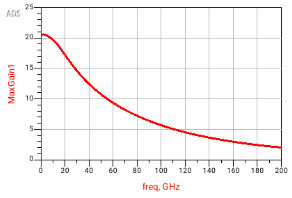
\includegraphics[width=\linewidth]{Design_figures/CBCE/SchematicCBCE_measureMaxGain.PNG}
    \caption{}
    \label{fig:SchematicCBCE_measureMaxGain}
    \end{subfigure}
    \hfill
    \begin{subfigure}{0.48\textwidth}
        \centering
        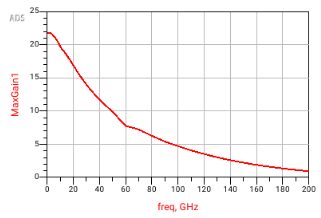
\includegraphics[width=\linewidth]{Design_figures/CBCE/LayoutCBCE_measureMaxGain.PNG}
        \caption{}
    \label{fig:LayoutCBCE_measureMaxGain}
    \end{subfigure}
    \caption{MaxGain measurement of the CECB in (a) schematic level and (b) layout level design}
\end{figure}
%%%%%%%%%%%%%%%%%%
\begin{comment}
    

\begin{figure}[hbt!]
    \centering
    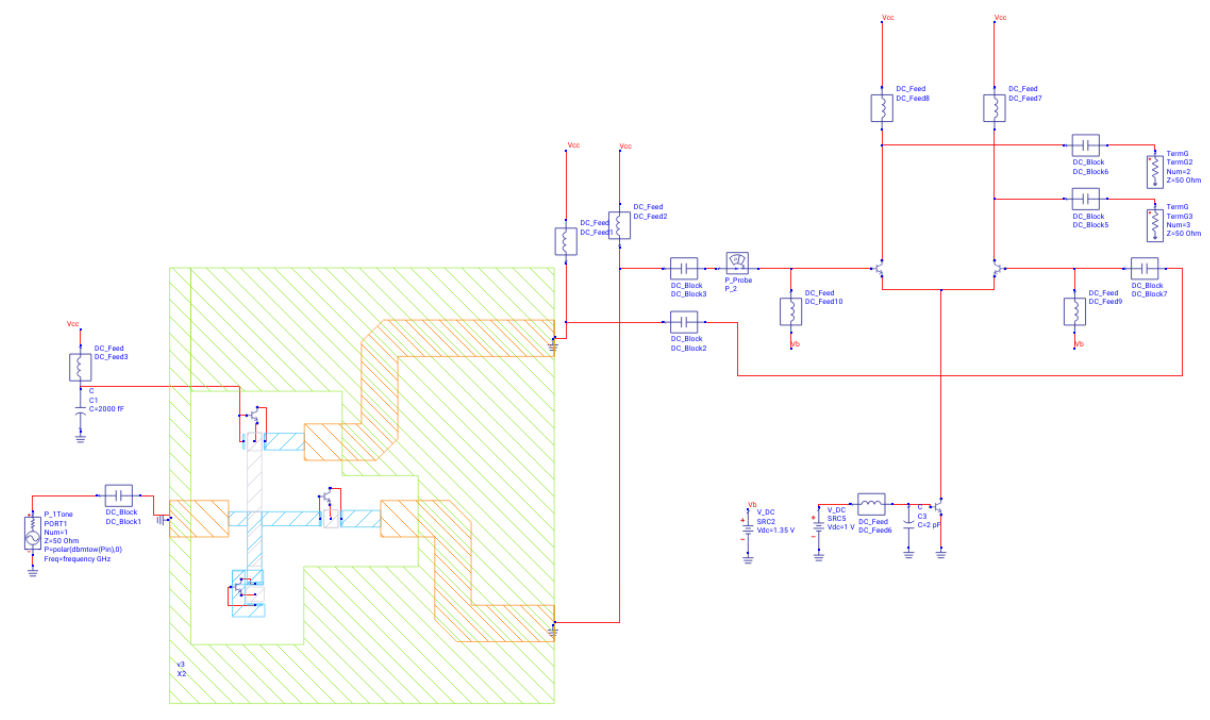
\includegraphics[width=1\linewidth]{Design_figures/CBCE/LayoutCBCE_&_diffential.PNG}
    \caption{Caption}
    \label{fig:placeholder}
\end{figure}


%%%%%%%%%%%%%%%%%%
\begin{figure}[H]
    \centering
    \begin{subfigure}[b]{0.48\linewidth}
        \centering
        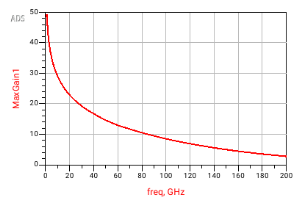
\includegraphics[width=\linewidth]{Design_figures/CBCE/LayoutCBCE_&_diffential_measureMaxGain.PNG}
        \caption{}
        \label{fig:placeholder}
    \end{subfigure}
    \hfill
    \begin{subfigure}[b]{0.48\linewidth}
        \centering
        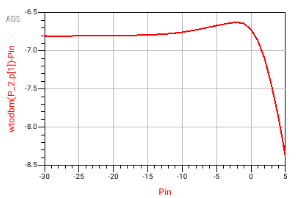
\includegraphics[width=\linewidth]{Design_figures/CBCE/LayoutCBCE_&_diffential_measureIP1dB.PNG}
        \caption{}
        \label{fig:placeholder}
    \end{subfigure}
    \caption{Caption}
    \label{fig:placeholder}
\end{figure}
%%%%%%%%%%%%%%%%%%
\begin{figure}[H]
    \centering
    \begin{subfigure}[b]{0.48\linewidth}
        \centering
        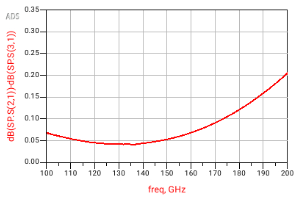
\includegraphics[width=\linewidth]{Design_figures/CBCE/LayoutCBCE_&_diffential_measureAmplitudeImbalance.PNG}
        \caption{}
        \label{fig:placeholder}
    \end{subfigure}
    \hfill
    \begin{subfigure}[b]{0.48\linewidth}
        \centering
        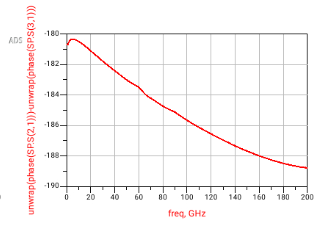
\includegraphics[width=\linewidth]{Design_figures/CBCE/LayoutCBCE_&_diffential_measurePhaseImbalance.PNG}
        \caption{}
        \label{fig:placeholder}
    \end{subfigure}
    \caption{Caption}
    \label{fig:placeholder}
\end{figure}
\end{comment}